

\begin{columns}
  \begin{column}{0.5\linewidth}
    \begin{center}
      \begin{tabular}{|M{0.4cm}|M{0.4cm}M{0.4cm}M{0.4cm}M{0.4cm}M{0.4cm}M{1.2cm}|}
        \hline
        $i$ & $r_i$ & $d_i$ & $W_i$ & $\bmin$ & $\bmax$ & $f_i(b)$\\[2mm]
        \hline
        1 & 0 & 2 & 6 & 3 & 3 & $b$\\[2mm]
        2 & 1 & 5 & 22 & 3 & 4 & $\rightarrow$ \\[2mm]
        3 & 0 & 6 & 39 & 1 & 5 & $3b+1$\\[2mm]
        \hline
        \multicolumn{7}{c}{}
      \end{tabular}
    \end{center}
  \end{column}
\hfill
    \begin{column}{0.4\linewidth}
\begin{tikzpicture}
[xscale=1,yscale=0.56]
\node (O) at (2,5) {};
\draw[->] (2,4) -- (5.5,4) node[below] {$b$}; 
\draw[dashed] (2,4) -- (2,5.5);
\draw[->] (2,5.5) -- (2,10) node[left] {$f_2(b)$};


\path[draw] (3,6) -- (4,8) -- (5,9) ;

\draw[dotted] (3,4) node[below] {\footnotesize $3$} -- (3,10);
\draw[dotted,color=gray!70] (4,4) node[below,color=black] {\footnotesize $4$}
-- (4,10);
\draw[dotted] (5,4) node[below] {\footnotesize $5$} -- (5,10);

\draw (2,6) node[left] {\footnotesize $6$};
\draw (2,8) node[left] {\footnotesize $8$};
\draw (2,9) node[left] {\footnotesize $9$};
\end{tikzpicture}
\end{column}
\end{columns}
\pause
  \begin{columns}
    \begin{column}{0.45\linewidth}
      \onslide<2->{
        \centering
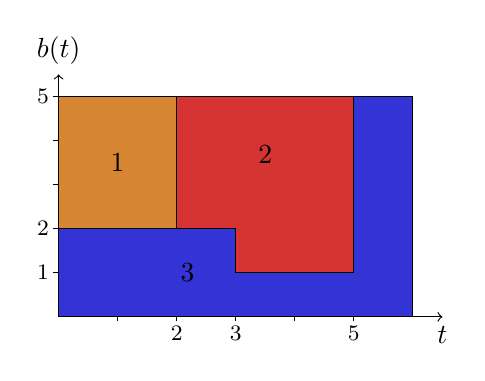
\begin{tikzpicture}
[xscale=0.75,yscale=0.56]
\node (O) at (0,0) {};
\draw[->] (0,0) -- (6.5,0) node[below] {$t$};
\draw[->] (0,0) -- (0,5.5) node[above] {$b(t)$};

\draw[fill=orange!80!black!80] (0,2) rectangle (2,5) node[midway] {$1$};
\path[draw,fill=blue!80!black!80] (0,0) -- (0,2) -- (3,2) -- (3,1) node[left=0.4cm] {$3$} -- (5,1) -- (5,5) -- (6,5)  -- (6,0) -- cycle;
\draw[fill=red!80!black!80] (2,5) -- (5,5) node[midway,below=0.5cm] {$2$} -- (5,1) -- (3,1) -- (3,2) -- (2,2) -- cycle;

\draw (0,1) node[left] {\footnotesize $1$};
\draw (0,2) node[left] {\footnotesize $2$};
\draw (0,5) node[left] {\footnotesize $5$};


\draw (2,0) node[below] {\footnotesize $2$};
\draw (3,0) node[below] {\footnotesize $3$};
\draw (5,0) node[below] {\footnotesize $5$};

\foreach \i in {1,...,5}{
\draw (\i,-0.1) -- (\i,0);
\draw (-0.1,\i) -- (0,\i);
}
\end{tikzpicture}

      }
    \end{column}
    \hfill
    \begin{column}{0.45\linewidth}
      \newbox\hautbox \setbox\hautbox=\hbox{\vphantom{\rule[-0.4cm]{0cm}{0.9cm}}}
      \begin{tabular}{@{\usebox{\hautbox}}l}
        \onslide<4->{$\int_0^{4} b_1(t)dt=?$} \\
        \onslide<5->{$\int_0^{2}${\color<5>{red!80!black!80}{$5$}}$dt$}\onslide<6->{$+\int_2^{4}${\color<6>{red!80!black!80}{$1$}}$dt$}\\
        \onslide<7->$=10+2=12$\\
      \end{tabular}
    \end{column}
    \hfill
  \end{columns}
